% Provenance (never printed): cycle 2 "Explorer les organisations du monde ---
% identifier des paysages" (littoraux, massifs montagneux, campagnes, villes),
% see sources/book1/PROVENANCE.md. Book 1, grade 1, chapter 2.
\chapter{As paisagens ao nosso redor}\label{ch:g1:landscapes-around-us}

Mia e o avô subiram até o alto da \omterm{def:g1:landscapes-around-us:landform}{colina} atrás da vila. Lá em cima, eles
se sentam na grama para recuperar o fôlego, e olham. Lá embaixo, os
telhados vermelhos da vila se apertam em volta da igreja. Um \omterm{def:g1:landscapes-around-us:water}{rio} faz
curvas entre campos verdes e amarelos e passa por baixo de uma ponte.
Há uma floresta escura na \omterm{def:g1:landscapes-around-us:landform}{colina} vizinha. E longe, bem longe, lá no fim
da terra, aparece uma faixa fina de azul.

``Aquilo é o mar'', diz o avô.

Tudo o que Mia consegue ver do alto da \omterm{def:g1:landscapes-around-us:landform}{colina}, perto e longe, é uma
\omterm{def:g1:landscapes-around-us:landscape}{paisagem}.

\begin{omfigure}
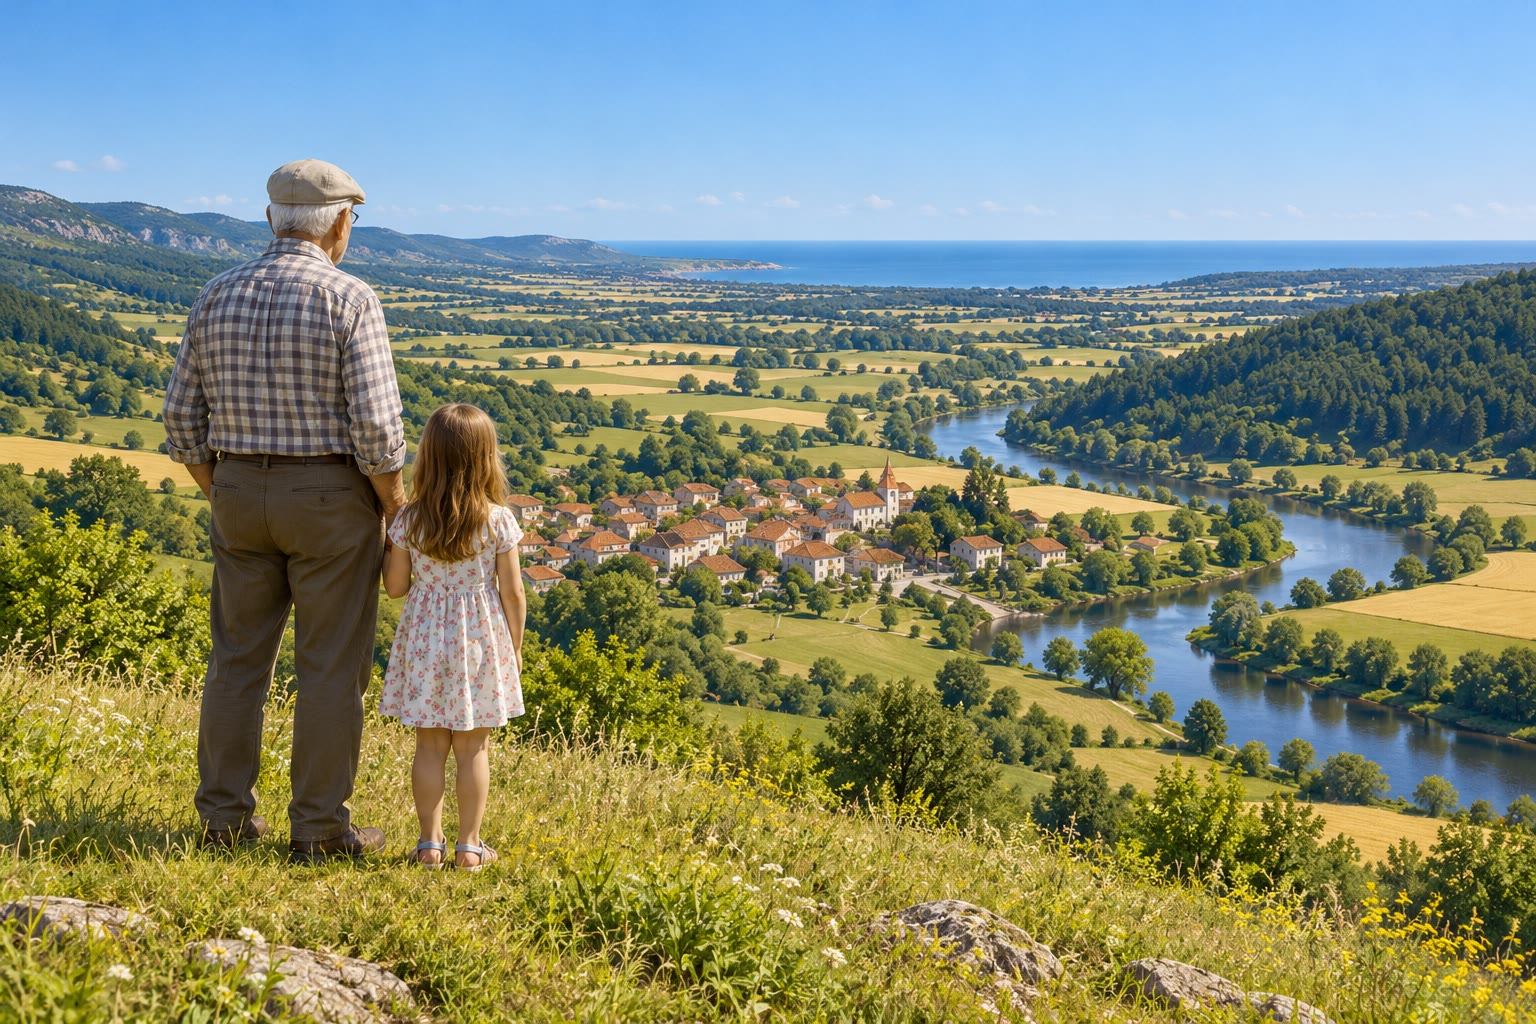
\includegraphics[width=0.72\linewidth]{images/book1/ai/g1-hilltop-view.jpg}

{\small Do alto de uma \omterm{def:g1:landscapes-around-us:landform}{colina}, vemos uma \omterm{def:g1:landscapes-around-us:landscape}{paisagem} inteira.}
\end{omfigure}

\section{O que é uma paisagem?}

\begin{definition}[Paisagem]\label{def:g1:landscapes-around-us:landscape}
Uma \emph{paisagem}\index{paisagem} é tudo o que vemos da terra com um só
olhar, desde onde estamos até o horizonte: a forma do terreno, a água,
as plantas e as coisas que as pessoas construíram.
\end{definition}

Uma \omterm{def:g1:landscapes-around-us:landscape}{paisagem} tem partes que estão perto e partes que estão longe. A parte
mais próxima de nós fica embaixo naquilo que vemos; ela parece grande e
vemos os seus detalhes. A parte distante fica em cima, perto do céu; ela
parece pequena e pálida.

\begin{omfigure}
\begin{tikzpicture}[x=1cm, y=1cm]
  \fill[ocBlue!12] (0,0) rectangle (10,5);
  % background: far hills
  \fill[black!18] (0,3.0) -- (1.5,3.6) -- (3,3.3) -- (5,3.9) -- (7,3.4) -- (8.5,3.8) -- (10,3.3) -- (10,2.9) -- (0,2.9) -- cycle;
  % middle: hills and fields
  \fill[green!35!omLithAlluv] (0,1.6) -- (2,2.4) -- (4,2.1) -- (6,2.7) -- (8,2.2) -- (10,2.5) -- (10,1.5) -- (0,1.5) -- cycle;
  \fill[green!25!omLithAlluv] (0,1.5) rectangle (10,2.95);
  \fill[green!35!omLithAlluv] (0,2.95) -- (2,3.1) -- (4,2.95) -- (6,3.25) -- (8,3.0) -- (10,3.1) -- (10,2.9) -- (0,2.9) -- cycle;
  \foreach \x in {5.6,5.9,6.2} \fill[red!55] (\x,2.25) -- ++(0.12,0.15) -- ++(0.12,-0.15) -- cycle;
  \foreach \x in {5.6,5.9,6.2} \fill[white] (\x+0.03,2.1) rectangle ++(0.18,0.15);
  % foreground
  \fill[green!55!black!60] (0,0) rectangle (10,1.5);
  \foreach \x in {0.8,2.1,8.6} {
    \fill[brown!70!black] (\x-0.06,0.4) rectangle (\x+0.06,0.9);
    \fill[green!45!black] (\x,1.15) circle (0.38);
  }
  % band borders and labels
  \draw[white, line width=1pt, dashed] (0,1.5) -- (10,1.5);
  \draw[white, line width=1pt, dashed] (0,2.95) -- (10,2.95);
  \node[font=\small\bfseries, fill=white, fill opacity=0.8, text opacity=1, inner sep=2pt] at (5,0.6) {primeiro plano: perto, grande, muitos detalhes};
  \node[font=\small\bfseries, fill=white, fill opacity=0.8, text opacity=1, inner sep=2pt] at (2.7,2.2) {plano intermediário};
  \node[font=\small\bfseries, fill=white, fill opacity=0.8, text opacity=1, inner sep=2pt] at (5,4.4) {plano de fundo: longe, pequeno, pálido};
\end{tikzpicture}

{\small Uma \omterm{def:g1:landscapes-around-us:landscape}{paisagem} vista em três faixas: o primeiro plano embaixo, o
plano intermediário e o plano de fundo, junto ao céu.}
\label{fig:g1:landscapes-around-us:bands}
\end{omfigure}

\section{As formas do terreno}

O chão não é plano em toda parte. Em alguns lugares ele sobe bem alto em
direção ao céu; em outros, desce formando depressões compridas; em outros
ainda, é plano até onde a vista alcança. Damos um nome a cada forma.

\begin{definition}[Formas de relevo]\label{def:g1:landscapes-around-us:landform}
Uma \emph{forma de relevo}\index{forma de relevo} é uma forma da superfície da terra.
\begin{itemize}
  \item Uma \emph{montanha}\index{montanha} é uma forma de relevo muito alta,
        de encostas íngremes; o seu ponto mais alto se chama cume. As
        montanhas mais altas têm neve no alto até no verão.
  \item Uma \emph{colina}\index{colina} é uma forma de relevo que se eleva
        acima do terreno em volta, mais baixa e mais arredondada que uma
        montanha.
  \item Um \emph{vale}\index{vale} é uma depressão comprida e baixa entre
        colinas ou montanhas; muitas vezes corre um \omterm{def:g1:landscapes-around-us:water}{rio} no fundo dele.
  \item Uma \emph{planície}\index{planicie@planície} é uma extensão de terra larga, plana e baixa.
\end{itemize}
\end{definition}

\begin{omfigure}
\begin{tikzpicture}[x=1cm, y=1cm]
  \fill[ocBlue!10] (0,0) rectangle (12.4,4.6);
  % sea
  \fill[omSea] (10.2,0) rectangle (12.4,0.55);
  % land profile: mountains, valley, hill, plain, coast
  \fill[omLithAlluv!80!green] (0,0) -- (0,2.2) -- (0.9,3.3) -- (1.5,3.0) -- (2.2,4.1)
     -- (2.9,2.6) -- (3.6,1.2) -- (3.9,0.9) -- (4.2,1.2) -- (5.0,2.0) -- (5.7,2.2)
     -- (6.4,1.6) -- (7.0,0.95) -- (8.0,0.8) -- (9.5,0.7) -- (10.2,0.6) -- (10.4,0.55)
     -- (10.4,0) -- cycle;
  \draw[black!60, line width=0.6pt] (0,2.2) -- (0.9,3.3) -- (1.5,3.0) -- (2.2,4.1)
     -- (2.9,2.6) -- (3.6,1.2) -- (3.9,0.9) -- (4.2,1.2) -- (5.0,2.0) -- (5.7,2.2)
     -- (6.4,1.6) -- (7.0,0.95) -- (8.0,0.8) -- (9.5,0.7) -- (10.2,0.6) -- (10.4,0.55);
  % snow caps
  \fill[white, draw=black!50, line width=0.3pt] (1.95,3.72) -- (2.2,4.1) -- (2.45,3.72) -- (2.3,3.78) -- (2.2,3.68) -- (2.08,3.78) -- cycle;
  \fill[white, draw=black!50, line width=0.3pt] (0.72,3.08) -- (0.9,3.3) -- (1.05,3.15) -- (0.9,3.12) -- cycle;
  % river in the valley
  \fill[omSea!90!black] (3.75,0.92) rectangle (4.05,0.98);
  % lake on the plain
  \fill[omSea] (7.6,0.82) ellipse (0.5 and 0.07);
  % village on the plain
  \foreach \x in {8.6,8.85,9.1} {
    \fill[white, draw=black!50, line width=0.3pt] (\x,0.74) rectangle ++(0.18,0.16);
    \fill[red!60] (\x-0.02,0.9) -- ++(0.11,0.12) -- ++(0.11,-0.12) -- cycle;
  }
  % labels
  \node[font=\small, above] at (2.2,4.12) {montanha};
  \node[font=\small, above] at (5.6,2.25) {colina};
  \node[font=\small] at (3.9,1.85) {vale};
  \node[font=\small, above] at (8.2,1.5) {planície};
  \draw[black!60, thin] (8.2,1.5) -- (8.2,0.85);
  \node[font=\small, align=center] at (11.3,1.4) {mar};
  \node[font=\scriptsize, below=2pt, fill=white, fill opacity=0.8, text opacity=1, inner sep=1pt] at (7.6,0.35) {lago};
  \draw[black!60, thin] (7.6,0.45) -- (7.6,0.78);
  \node[font=\scriptsize, below=2pt, fill=white, fill opacity=0.8, text opacity=1, inner sep=1pt] at (10.3,0.35) {litoral};
  \node[font=\scriptsize, fill=white, fill opacity=0.8, text opacity=1, inner sep=1pt] at (3.9,0.2) {rio};
  \draw[black!60, thin] (3.9,0.32) -- (3.9,0.88);
\end{tikzpicture}

{\small As formas do terreno, das \omterm{def:g1:landscapes-around-us:landform}{montanhas} até o mar, vistas de lado (as
alturas estão desenhadas muito maiores do que são na realidade).}
\label{fig:g1:landscapes-around-us:profile}
\end{omfigure}

\begin{omfigure}
\begin{minipage}[b]{0.49\linewidth}\centering
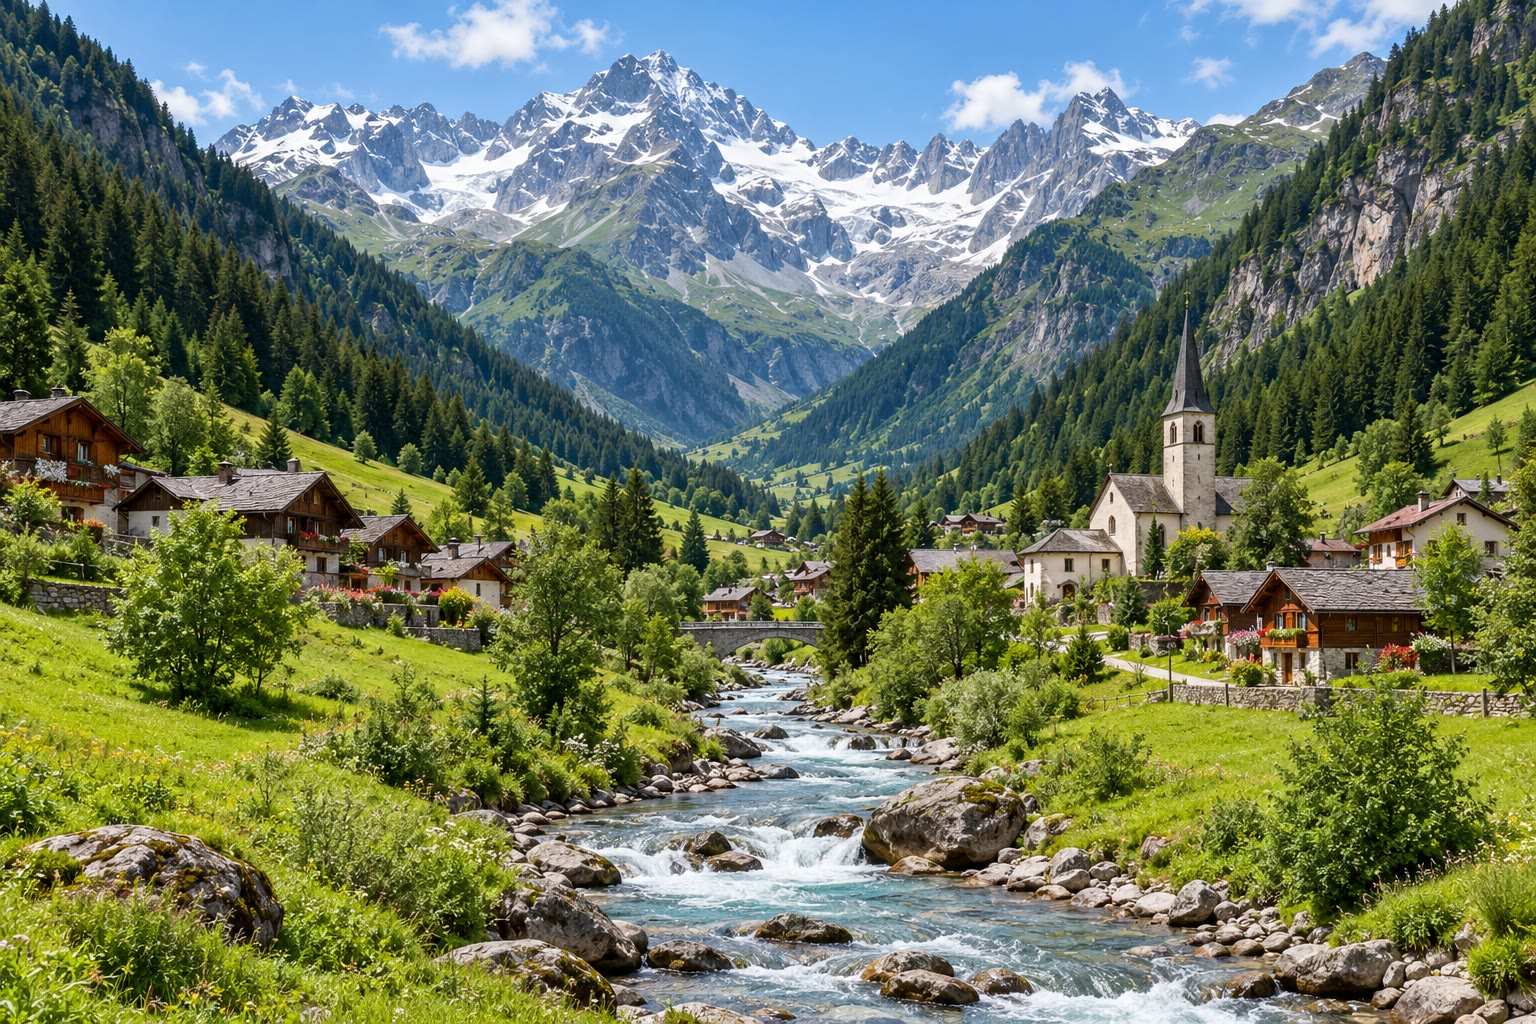
\includegraphics[width=\linewidth]{images/book1/ai/g1-mountain-village.jpg}

{\small \omterm{def:g1:landscapes-around-us:landform}{Montanhas} e uma vila no \omterm{def:g1:landscapes-around-us:landform}{vale} entre elas.}
\end{minipage}\hfill
\begin{minipage}[b]{0.49\linewidth}\centering
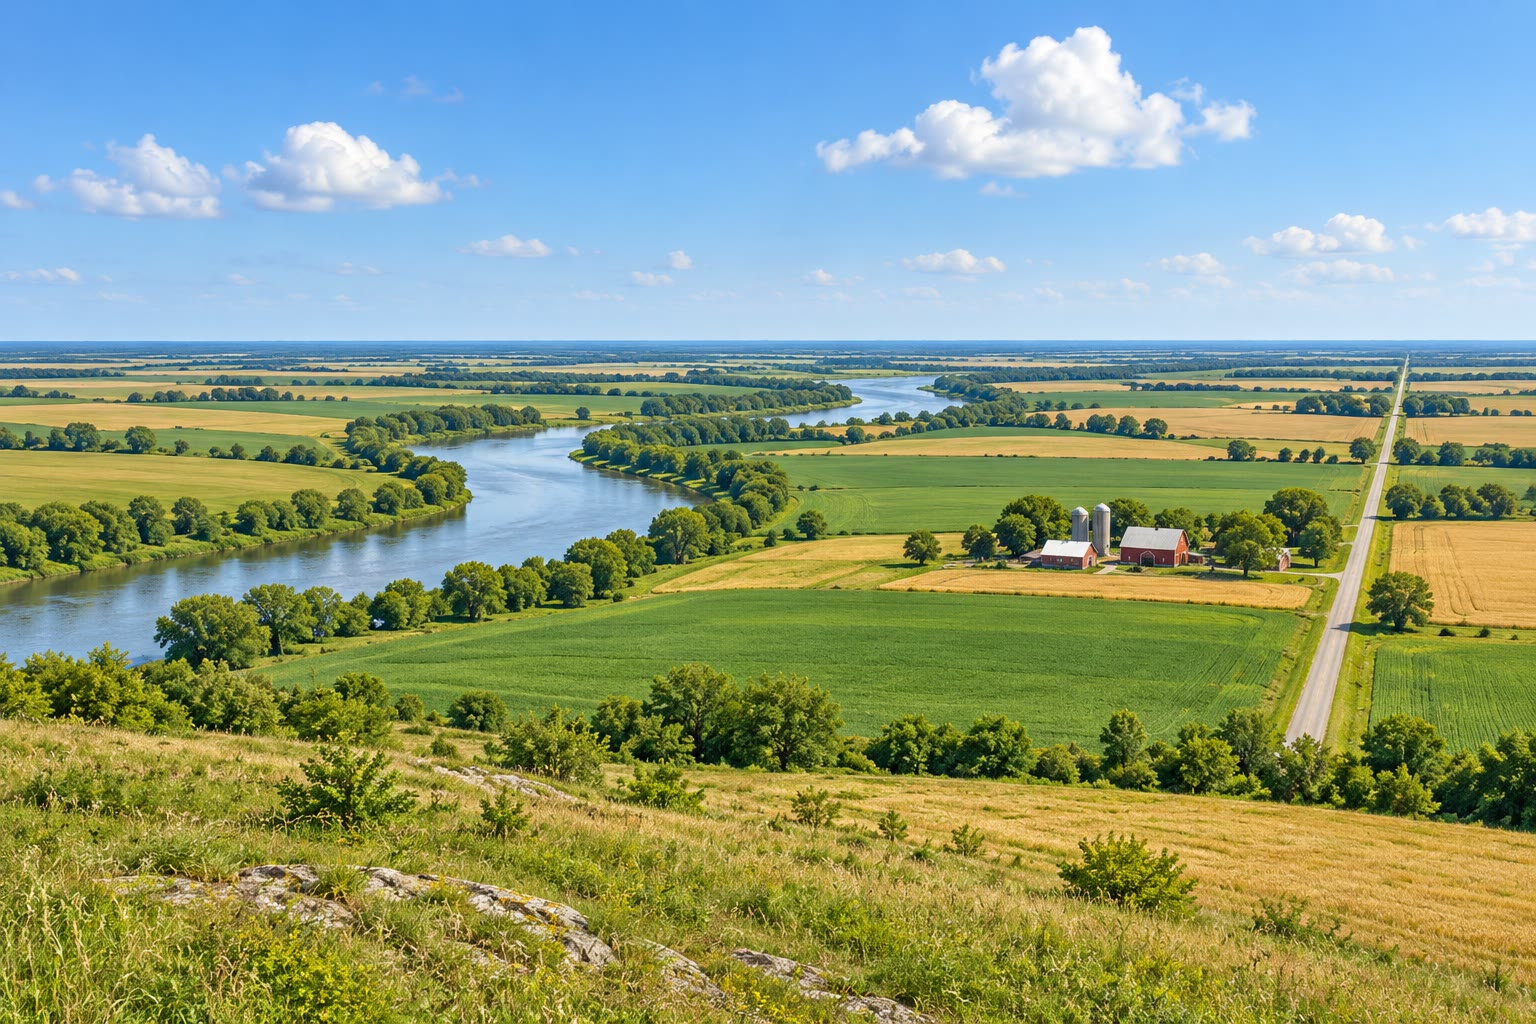
\includegraphics[width=\linewidth]{images/book1/ai/g1-plain-river.jpg}

{\small Uma \omterm{def:g1:landscapes-around-us:landform}{planície}, com um \omterm{def:g1:landscapes-around-us:water}{rio} e plantações.}
\end{minipage}
\end{omfigure}

\begin{example}[Montanha ou colina?]\label{ex:g1:landscapes-around-us:mountain-hill}
Não existe uma altura exata a partir da qual uma \omterm{def:g1:landscapes-around-us:landform}{colina} vira \omterm{def:g1:landscapes-around-us:landform}{montanha}.
Olhamos a forma: uma \omterm{def:g1:landscapes-around-us:landform}{montanha} é alta e íngreme, muitas vezes rochosa, às
vezes com neve no alto; uma \omterm{def:g1:landscapes-around-us:landform}{colina} é mais baixa e mais arredondada, muitas
vezes coberta de grama, de plantações ou de mato, e dá para chegar ao
alto dela a pé em pouco tempo.
\end{example}

\section{A água na paisagem}

A água faz parte da maioria das \omterm{def:g1:landscapes-around-us:landscape}{paisagens}. Ela desce das \omterm{def:g1:landscapes-around-us:landform}{colinas} e das
\omterm{def:g1:landscapes-around-us:landform}{montanhas}, junta-se nas partes baixas e chega ao mar.

\begin{definition}[A água numa paisagem]\label{def:g1:landscapes-around-us:water}
Um \emph{rio}\index{rio} é uma água que corre sem parar num canal
comprido, de um terreno mais alto até um lago ou até o mar. Um
\emph{lago}\index{lago} é uma grande extensão de água cercada de terra. O
\emph{litoral}\index{litoral} é o lugar onde a terra encontra o mar.
\end{definition}

\begin{omfigure}
\begin{minipage}[b]{0.49\linewidth}\centering
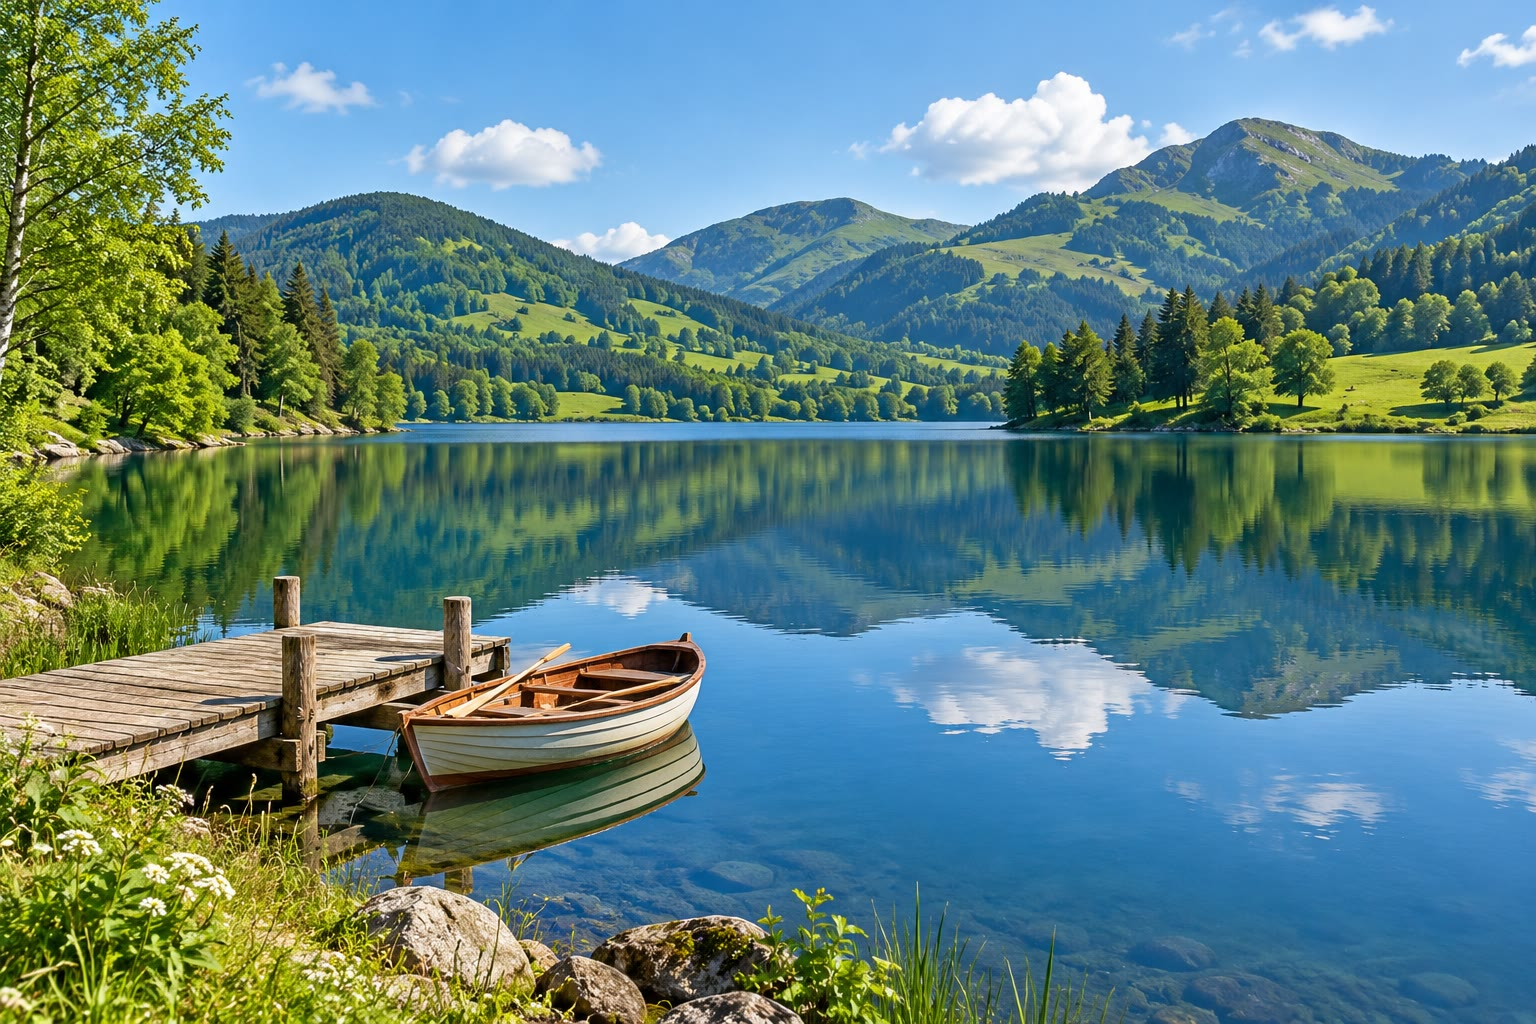
\includegraphics[width=\linewidth]{images/book1/ai/g1-lake-hills.jpg}

{\small Um \omterm{def:g1:landscapes-around-us:water}{lago} entre \omterm{def:g1:landscapes-around-us:landform}{colinas}.}
\end{minipage}\hfill
\begin{minipage}[b]{0.49\linewidth}\centering
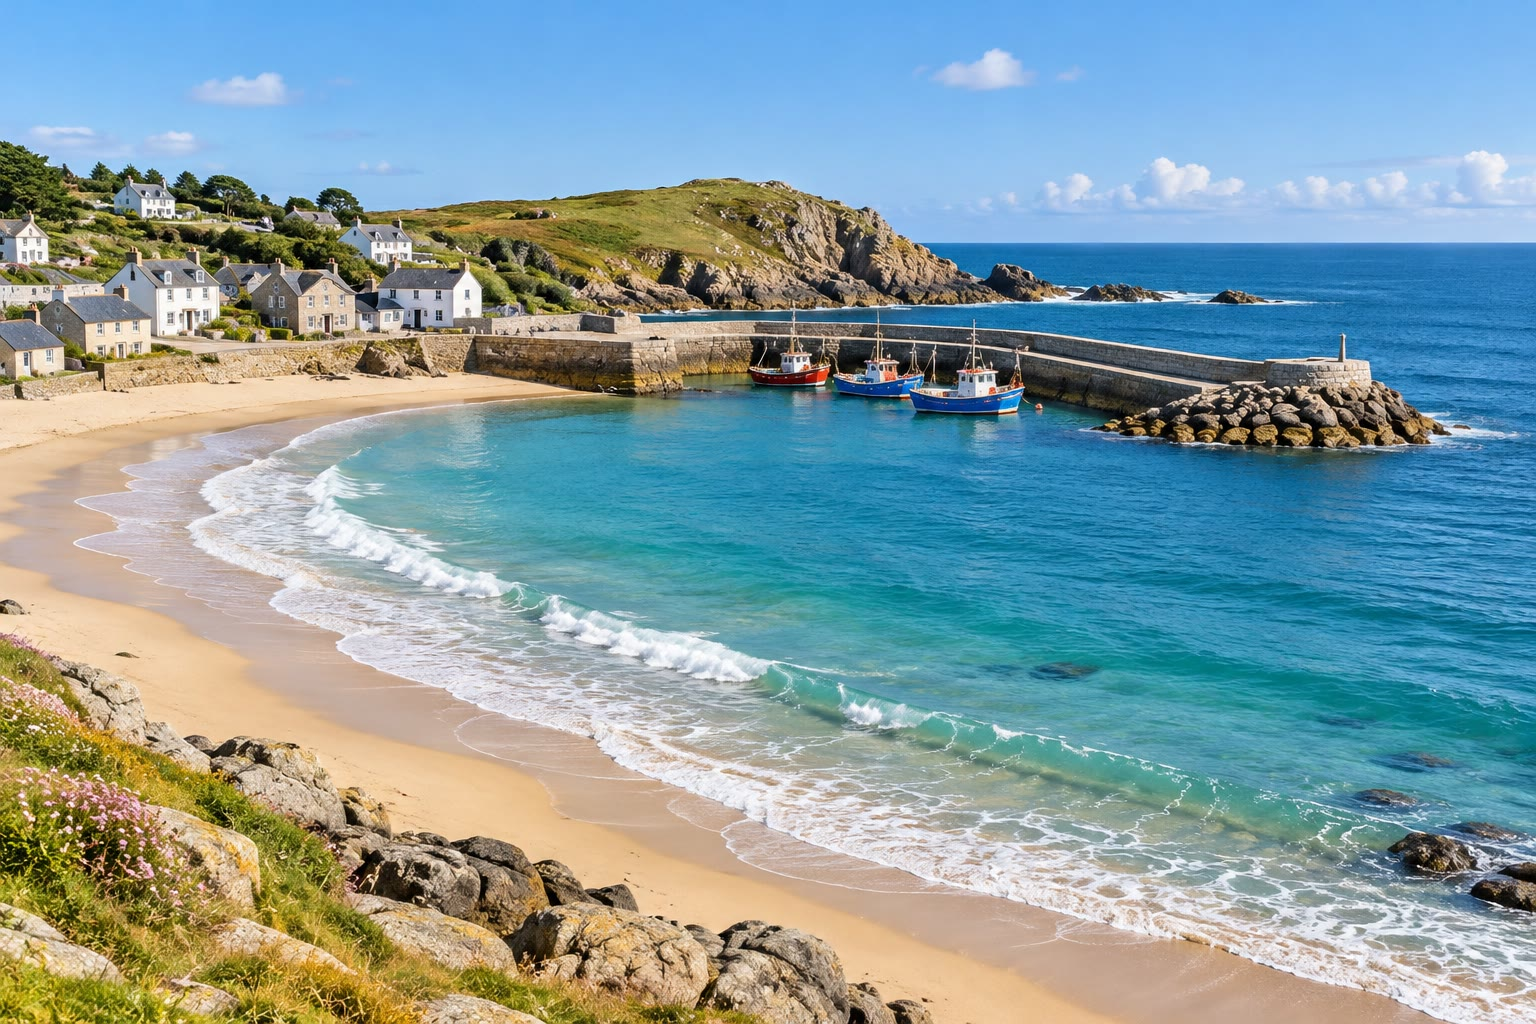
\includegraphics[width=\linewidth]{images/book1/ai/g1-coast-harbour.jpg}

{\small Um \omterm{def:g1:landscapes-around-us:water}{litoral}: uma praia, rochedos e um porto.}
\end{minipage}
\end{omfigure}

\begin{remark}[A água sempre desce]\label{rem:g1:landscapes-around-us:downhill}
Um \omterm{def:g1:landscapes-around-us:water}{rio} sempre corre de um terreno mais alto para um terreno mais baixo. É
por isso que os \omterm{def:g1:landscapes-around-us:water}{rios} correm no fundo dos \omterm{def:g1:landscapes-around-us:landform}{vales} e que, no fim, chegam a um
\omterm{def:g1:landscapes-around-us:water}{lago} ou ao mar, que ficam mais baixos que a terra em volta.
\end{remark}

\section{Partes naturais e partes construídas}

Algumas partes de uma \omterm{def:g1:landscapes-around-us:landscape}{paisagem} já estavam lá antes das pessoas chegarem:
as \omterm{def:g1:landscapes-around-us:landform}{montanhas}, os \omterm{def:g1:landscapes-around-us:water}{rios}, as florestas. Outras partes foram feitas pelas
pessoas: casas, estradas, pontes, plantações.

\begin{definition}[Partes naturais e partes construídas]\label{def:g1:landscapes-around-us:natural-built}
Um \emph{elemento natural}\index{elemento natural} de uma \omterm{def:g1:landscapes-around-us:landscape}{paisagem} é uma parte
que não foi feita pelas pessoas: uma \omterm{def:g1:landscapes-around-us:landform}{montanha}, um \omterm{def:g1:landscapes-around-us:water}{rio}, um \omterm{def:g1:landscapes-around-us:water}{lago}, uma floresta, uma praia.
Um \emph{elemento construído}\index{elemento construido@elemento construído} é uma parte feita ou modificada pelas
pessoas: uma casa, uma estrada, uma ponte, um porto, uma plantação, um jardim.
\end{definition}

\begin{omfigure}
\begin{tikzpicture}[x=1cm, y=1cm]
  \node[draw=omDef!80!black, fill=omDef!10, rounded corners, text width=5.2cm,
        align=left, minimum height=3.2cm, anchor=north] (n) at (0,0)
    {\textbf{natural}\\[2pt] montanha\\ colina\\ vale\\ rio\\ lago\\ floresta\\ praia};
  \node[draw=omMeth!80!black, fill=omMeth!10, rounded corners, text width=5.2cm,
        align=left, minimum height=3.2cm, anchor=north] (b) at (6,0)
    {\textbf{construído pelas pessoas}\\[2pt] casa\\ igreja\\ estrada\\ ponte\\ porto\\ plantação\\ jardim};
\end{tikzpicture}

{\small Separando as partes da \omterm{def:g1:landscapes-around-us:landscape}{paisagem} de Mia. Uma plantação é construída:
as pessoas limparam o terreno e plantaram.}
\label{fig:g1:landscapes-around-us:sort}
\end{omfigure}

\section{As paisagens mudam}

Uma \omterm{def:g1:landscapes-around-us:landscape}{paisagem} não fica igual para sempre. Algumas mudanças são rápidas, e
outras são tão lentas que ninguém as percebe ao longo de uma vida inteira.
\begin{itemize}
  \item \textbf{Com as estações:} os campos ficam marrons depois de arados,
        verdes na primavera, dourados antes da colheita; as árvores perdem
        as folhas no outono; a neve pode cobrir tudo no inverno.
  \item \textbf{Por causa das pessoas:} uma vila cresce e vira cidade; uma
        floresta é derrubada para fazer plantações; uma estrada nova e uma
        ponte atravessam o \omterm{def:g1:landscapes-around-us:landform}{vale}.
  \item \textbf{Por causa da água e do \omterm{def:g1:watching-the-weather:weather}{tempo}:} depois de uma grande
        tempestade, um \omterm{def:g1:landscapes-around-us:water}{rio} pode sair do seu leito e cobrir os campos por
        alguns dias; no \omterm{def:g1:landscapes-around-us:water}{litoral}, as ondas desgastam as rochas devagar.
\end{itemize}

\begin{omfigure}
\begin{tikzpicture}[x=1cm, y=1cm]
  \foreach \k/\t in {0/antigamente, 1/hoje} {
  \begin{scope}[shift={(\k*6.4,0)}]
    \fill[ocBlue!8] (0,0) rectangle (5.8,3.4);
    \fill[green!30!omLithAlluv] (0,0) rectangle (5.8,1.9);
    % river
    \fill[omSea] (0,0.55) .. controls (1.5,0.9) and (2.5,0.2) .. (5.8,0.6)
       -- (5.8,0.85) .. controls (2.5,0.45) and (1.5,1.15) .. (0,0.8) -- cycle;
    % hill
    \fill[green!45!black!55] (2.8,1.9) .. controls (3.8,3.1) and (4.8,3.1) .. (5.8,2.2) -- (5.8,1.9) -- cycle;
    \ifnum\k=0
      % forest everywhere, a few houses
      \foreach \x in {0.4,0.9,1.4,1.9,2.4,4.3,4.8,5.3}
        \fill[green!40!black] (\x,1.45) circle (0.22);
      \foreach \x in {3.4,3.75} {
        \fill[white, draw=black!50, line width=0.3pt] (\x,1.15) rectangle ++(0.24,0.2);
        \fill[red!60] (\x-0.03,1.35) -- ++(0.15,0.14) -- ++(0.15,-0.14) -- cycle; }
    \else
      % fields, many houses, a road and a bridge
      \foreach \x/\c in {0.1/yellow!60, 1.3/green!55, 4.5/yellow!45}
        \fill[\c] (\x,1.05) rectangle ++(1.1,0.5);
      \fill[black!35] (2.65,0) rectangle (2.95,1.9);
      \fill[black!55] (2.55,0.5) rectangle (3.05,0.9);
      \foreach \x in {3.2,3.55,3.9} \foreach \y in {1.1,1.45} {
        \fill[white, draw=black!50, line width=0.3pt] (\x,\y) rectangle ++(0.24,0.2);
        \fill[red!60] (\x-0.03,\y+0.2) -- ++(0.15,0.14) -- ++(0.15,-0.14) -- cycle; }
      \foreach \x in {4.6,5.2} \fill[green!40!black] (\x,2.35) circle (0.2);
    \fi
    \node[font=\small\bfseries] at (2.9,-0.3) {\t};
  \end{scope}}
\end{tikzpicture}

{\small O mesmo \omterm{def:g1:landscapes-around-us:landform}{vale} antigamente e hoje. A \omterm{def:g1:landscapes-around-us:landform}{colina} e o \omterm{def:g1:landscapes-around-us:water}{rio} não saíram do
lugar; as pessoas derrubaram a maior parte da floresta, fizeram
plantações, construíram mais casas, uma estrada e uma ponte.}
\label{fig:g1:landscapes-around-us:change}
\end{omfigure}

\begin{example}[Cidade e campo]\label{ex:g1:landscapes-around-us:town}
Numa cidade, quase tudo o que vemos foi construído: ruas, casas, lojas,
pontes, parques. No campo vemos principalmente plantações, matas e
pastos, com alguns sítios e vilas. As duas são \omterm{def:g1:landscapes-around-us:landscape}{paisagens}. Mesmo no meio
de uma cidade grande as formas do terreno continuam lá: um \omterm{def:g1:landscapes-around-us:water}{rio} atravessa
a cidade, e algumas ruas sobem uma \omterm{def:g1:landscapes-around-us:landform}{colina}.
\end{example}

\section{Descrever uma paisagem}

\begin{method}[Descrever uma paisagem em quatro passos]\label{met:g1:landscapes-around-us:describe}
Para descrever uma \omterm{def:g1:landscapes-around-us:landscape}{paisagem}, do alto de uma \omterm{def:g1:landscapes-around-us:landform}{colina} ou numa foto:
\begin{enumerate}
  \item \textbf{Divida-a em três faixas:} o primeiro plano, o plano
        intermediário e o plano de fundo.
  \item \textbf{Dê nome às formas do terreno:} \omterm{def:g1:landscapes-around-us:landform}{montanhas}, \omterm{def:g1:landscapes-around-us:landform}{colinas}, \omterm{def:g1:landscapes-around-us:landform}{vales},
        \omterm{def:g1:landscapes-around-us:landform}{planícies}.
  \item \textbf{Encontre a água:} um \omterm{def:g1:landscapes-around-us:water}{rio}, um \omterm{def:g1:landscapes-around-us:water}{lago}, o mar e o seu \omterm{def:g1:landscapes-around-us:water}{litoral}.
  \item \textbf{Encontre o que as pessoas construíram:} casas, estradas,
        pontes, plantações.
\end{enumerate}
\end{method}

\begin{example}[A paisagem de Mia]\label{ex:g1:landscapes-around-us:mia}
No primeiro plano, a grama do alto da \omterm{def:g1:landscapes-around-us:landform}{colina}. No plano intermediário, um
\omterm{def:g1:landscapes-around-us:landform}{vale} com um \omterm{def:g1:landscapes-around-us:water}{rio}, uma ponte e uma vila, com plantações em volta, e uma
floresta na \omterm{def:g1:landscapes-around-us:landform}{colina} vizinha. No plano de fundo, uma \omterm{def:g1:landscapes-around-us:landform}{planície} e, no fim da
terra, o \omterm{def:g1:landscapes-around-us:water}{litoral} e o mar. Naturais: as \omterm{def:g1:landscapes-around-us:landform}{colinas}, o \omterm{def:g1:landscapes-around-us:landform}{vale}, o \omterm{def:g1:landscapes-around-us:water}{rio}, a floresta,
o mar. Construídos: a vila, a igreja, a ponte, as plantações.
\end{example}

\section{Exercícios}

\begin{exercise}[$\star$]\label{exo:g1:landscapes-around-us:1}
Dê o nome das quatro formas do terreno que você aprendeu neste capítulo.
\end{exercise}

\begin{exercise}[$\star$]\label{exo:g1:landscapes-around-us:2}
O que é mais alto e mais íngreme: uma \omterm{def:g1:landscapes-around-us:landform}{colina} ou uma \omterm{def:g1:landscapes-around-us:landform}{montanha}?
\end{exercise}

\begin{exercise}[$\star$]\label{exo:g1:landscapes-around-us:3}
Natural ou construído? Um \omterm{def:g1:landscapes-around-us:water}{rio}; uma estrada; uma floresta; uma ponte; uma praia; uma casa.
\end{exercise}

\begin{exercise}[$\star$]\label{exo:g1:landscapes-around-us:4}
Onde fica o \omterm{def:g1:landscapes-around-us:water}{litoral}: onde a terra encontra um \omterm{def:g1:landscapes-around-us:water}{rio}, ou onde a terra
encontra o mar?
\end{exercise}

\begin{exercise}[$\star$]\label{exo:g1:landscapes-around-us:5}
Observe a foto das \omterm{def:g1:landscapes-around-us:landform}{montanhas} e da sua vila. Dê o nome de um \omterm{def:g1:landscapes-around-us:natural-built}{elemento
natural} e de um \omterm{def:g1:landscapes-around-us:natural-built}{elemento construído}.
\end{exercise}

\begin{exercise}[$\star$]\label{exo:g1:landscapes-around-us:6}
No desenho das formas do terreno, qual \omterm{def:g1:landscapes-around-us:landform}{forma de relevo} é a mais alta? Por
onde corre o \omterm{def:g1:landscapes-around-us:water}{rio}?
\end{exercise}

\begin{exercise}[$\star\star$]\label{exo:g1:landscapes-around-us:7}
De onde vem um \omterm{def:g1:landscapes-around-us:water}{rio}, e para onde ele vai? Por que ele nunca corre para
cima, até o alto de uma \omterm{def:g1:landscapes-around-us:landform}{colina}?
\end{exercise}

\begin{exercise}[$\star\star$]\label{exo:g1:landscapes-around-us:8}
Numa foto de uma \omterm{def:g1:landscapes-around-us:landscape}{paisagem}, uma árvore na parte de baixo da foto parece
maior do que uma \omterm{def:g1:landscapes-around-us:landform}{colina} inteira lá em cima. Por quê?
\end{exercise}

\begin{exercise}[$\star\star$]\label{exo:g1:landscapes-around-us:9}
Descreva a foto da \omterm{def:g1:landscapes-around-us:landform}{planície} com o seu \omterm{def:g1:landscapes-around-us:water}{rio} em três faixas: o que há no
primeiro plano, no plano intermediário e no plano de fundo?
\end{exercise}

\begin{exercise}[$\star\star$]\label{exo:g1:landscapes-around-us:10}
Uma plantação de trigo é verde ou dourada, como a grama. Por que dizemos
que ela é um \omterm{def:g1:landscapes-around-us:natural-built}{elemento construído} da \omterm{def:g1:landscapes-around-us:landscape}{paisagem}, e não um \omterm{def:g1:landscapes-around-us:natural-built}{elemento natural}?
\end{exercise}

\begin{exercise}[$\star\star$]\label{exo:g1:landscapes-around-us:11}
Observe o desenho do \omterm{def:g1:landscapes-around-us:landform}{vale} antigamente e hoje. Dê o nome de duas coisas que
não mudaram e de três coisas que as pessoas acrescentaram.
\end{exercise}
